% THIS IS AN EXAMPLE DOCUMENT FOR VLDB 2012
% based on ACM SIGPROC-SP.TEX VERSION 2.7
% Modified by  Gerald Weber <gerald@cs.auckland.ac.nz>
% Removed the requirement to include *bbl file in here. (AhmetSacan, Sep2012)
% Fixed the equation on page 3 to prevent line overflow. (AhmetSacan, Sep2012)


\documentclass{vldb}
\usepackage{graphicx}
\usepackage{enumitem}

\usepackage{pgfplots}
\pgfplotsset{compat=1.16}

\usepackage{balance}  % for  \balance command ON LAST PAGE  (only there!)
\usepackage{array}

\usepackage[hyphens]{url}

% % The following was an attempt to make it possible to specify -shade to tla2tex.TLA but \setboolean{shading}{true} doesn't actually render a gray box.
% % \usepackage{color}
% % \definecolor{boxshade}{gray}{0.85}
% \usepackage{tlatex}
% % Another option would be to convert the Trace.tex and array_ot*.tex file to .pdf files and embed them directly.
% % Embedding the .pdf files directly is the chosen approach. It required
% % 1. Running `java -cp '/Applications/TLA+ Toolbox.app/Contents/Eclipse/tla2tools.jar' tla2tex.TLA -style tlatex -shade -nops myspec.tla`
% % 2. Editing the generated myspec.tex to say
% %    \documentclass[varwidth=19pc, border={6pt 0pt 6pt 0pt}]{standalone}
% %    in place of \documentclass{article}.
% %    Doing so causes the generated PDF file to be sized according to the column width. Originally started with 42pc / 2 = 21pc but then the text wrapping slightly differed from having the .tex file contents embedded, so shrunk the column width for the generated PDF slightly further.
% % 3. Running pdflatex myspec.tex to generate myspec.pdf.


% Include information below and uncomment for camera ready
\vldbTitle{eXtreme Modelling in Practice}
\vldbAuthors{A. Jesse Jiryu Davis, Max Hirschhorn, Judah Schvimer}
\vldbDOI{https://doi.org/10.14778/3397230.3397233}
\vldbVolume{13}
\vldbNumber{9}
\vldbYear{2020}

\begin{document}

% \tolerance 9999
\emergencystretch 3em

% ****************** TITLE ****************************************

\title{eXtreme Modelling in Practice}
% OUTLINE: https://docs.google.com/document/d/16qDw3hxpi64ASPm0j0HneQSjyY7Kf93tCCLzG1NdOFM/edit

% possible, but not really needed or used for PVLDB:
%\subtitle{[Extended Abstract]
%\titlenote{A full version of this paper is available as\textit{Author's Guide to Preparing ACM SIG Proceedings Using \LaTeX$2_\epsilon$\ and BibTeX} at \texttt{www.acm.org/eaddress.htm}}}

% ****************** AUTHORS **************************************

% You need the command \numberofauthors to handle the 'placement
% and alignment' of the authors beneath the title.
%
% For aesthetic reasons, we recommend 'three authors at a time'
% i.e. three 'name/affiliation blocks' be placed beneath the title.
%
% NOTE: You are NOT restricted in how many 'rows' of
% "name/affiliations" may appear. We just ask that you restrict
% the number of 'columns' to three.
%
% Because of the available 'opening page real-estate'
% we ask you to refrain from putting more than six authors
% (two rows with three columns) beneath the article title.
% More than six makes the first-page appear very cluttered indeed.
%
% Use the \alignauthor commands to handle the names
% and affiliations for an 'aesthetic maximum' of six authors.
% Add names, affiliations, addresses for
% the seventh etc. author(s) as the argument for the
% \additionalauthors command.
% These 'additional authors' will be output/set for you
% without further effort on your part as the last section in
% the body of your article BEFORE References or any Appendices.

\numberofauthors{3} %  
\author{
% The command \alignauthor (no curly braces needed) should
% precede each author name, affiliation/snail-mail address and
% e-mail address. Additionally, tag each line of
% affiliation/address with \affaddr, and tag the
% e-mail address with \email.
%
% 1st. author
\alignauthor
A. Jesse Jiryu Davis\\
       \affaddr{MongoDB, Inc.}\\
       \affaddr{1633 Broadway}\\
       \affaddr{New York, NY 10019}\\
       \email{jesse@mongodb.com}
% 2nd. author
\alignauthor
Max Hirschhorn\\
       \affaddr{MongoDB, Inc.}\\
       \affaddr{1633 Broadway}\\
       \affaddr{New York, NY 10019}\\
       \email{max.hirschhorn @mongodb.com}
% 3rd. author
\alignauthor
Judah Schvimer\\
       \affaddr{MongoDB, Inc.}\\
       \affaddr{1633 Broadway}\\
       \affaddr{New York, NY 10019}\\
       \email{judah@mongodb.com}
}
% There's nothing stopping you putting the seventh, eighth, etc.
% author on the opening page (as the 'third row') but we ask,
% for aesthetic reasons that you place these 'additional authors'
% in the \additional authors block, viz.

% Just remember to make sure that the TOTAL number of authors
% is the number that will appear on the first page PLUS the
% number that will appear in the \additionalauthors section.

\maketitle

% \pagestyle{empty} suppresses the page numbers.
% When we are informed of the page numbers in the second round, \setcounter{page}{1} can be used to set the starting page.
% (presumably we'll update the "xxxx-yyyy" in the vldb.cls itself?)
\pagestyle{empty}
% \setcounter{page}{1}

% ********************************************************************
% ****************** Abstract ****************************************
% ********************************************************************
\begin{abstract}
Formal modelling is a powerful tool for developing complex systems. 
At MongoDB, we use TLA+ to model and verify multiple aspects of different systems. 
Ensuring conformance between a specification and its implementation can add value to any specification; it can avoid transcription errors, prevent bugs in large organizations rapidly developing the specified code, and even keep multiple implementations of the same specification in sync.
In this paper, we explore model-based testing as a tool for ensuring specification-implementation conformance.
We attempted two case studies: model-based trace-checking (MBTC) in the MongoDB Server's replication protocol and model-based test-case generation (MBTCG) in MongoDB Realm Sync's operational transformation algorithm.
We found MBTC to be impractical as a required component of development of the Server. 
MBTCG was highly successful for Realm Sync, however.
We analyze why one technique succeeded and the other failed, and advise future implementers making similar attempts at model-based testing.
\end{abstract}

% ********************************************************************
% ****************** Introduction ************************************
% ********************************************************************
\section{Introduction}
\label{sec:introduction}

It is well established that formal modelling catches bugs, aids software design, and improves code quality \cite{Newcombe2014UseOfFormalMethodsAmazon}.
Formal methods are increasingly being used to gain confidence in mission-critical, highly complex systems in multiple domains across many companies. 
Amazon \cite{Newcombe2014UseOfFormalMethodsAmazon, Chudnov18AmazonS2N, Cook18SecurityAWS}, Intel \cite{Kaivola09IntelI7, Beers08IntelExperience}, Microsoft \cite{Shukla18AzureCosmosDB}, and Springer Verlag \cite{Neubauer12AutomatedContinuousQualityAssurance}, have all written about their uses of formal methods and the value they've gained from modelling and verifying industrial software. 
But software engineers in industry are often skeptical of the value of the model unless it can be shown to match the implementation \cite{Wayne18AgileFormalMethods, Newcombe2014UseOfFormalMethodsAmazon}, due to the risk of concurrency simplifications that do not reflect the real system and \textit{transcription bugs}; that is, logic bugs due to mistakes in the implementation of the specification.
Further, it can be difficult to ensure that in a large engineering organization, changes in the production code are accompanied by changes in the model of the code.

\textit{eXtreme Modelling}, in which ``model and implementation are developed in parallel'' \cite{Gravell11ConcurrentDevelopmentOfModelAndImplementation}, has been proposed to prevent implementations and specifications from diverging.
Of the several guidelines included in this method, we attempted the following:
\begin{enumerate}[itemsep=-0.5ex]
  \item Multiple specifications model aspects of the system
  \item Models are written just prior to the implementation
  \item Models evolve with the implementation
  \item Tests are generated from the model and/or trace-checking verifies that test traces are legal in the model
\end{enumerate}

Although eXtreme Modelling was not intended for existing code bases and specifications, we attempted to lay the groundwork to use this technique on future projects in which we would write the specification before the implementation, and future code changes could affect the code's conformance with its specification.

\subsection{Contributions}

We undertook two case studies, using two existing code bases.
We attempted model-based trace-checking (MBTC) in the MongoDB Server.
One of our requirements was that the marginal cost of implementing MBTC for each future specification should be cheap, following an initial investment in trace-checking infrastructure.
After a great deal of effort, we determined that future specifications would not be easily trace-checked, and decided MBTC was impractical for the MongoDB Server.
The system's enormous code size and complex internal concurrency control were the main impediments.
In MongoDB Realm Sync, we succeeded in using model-based test-case generation (MBTCG) to ensure conformance between an existing implementation, a newly written specification, and a subsequent implementation of the same specification in a different programming language.

This paper will show what factors made MBTCG successful and MBTC unsuccessful.
This paper will identify lessons learned in both techniques and avenues of future research to make MBTC more practical.

This paper provides background to this research in Section \ref{sec:background}. 
Section \ref{sec:related_work} reviews related work. 
Section \ref{sec:model_based_trace_checking} describes our attempt at MBTC, and the challenges met. 
\ref{sec:model_based_test_case_generation} describes our success with MBTCG. 
Finally, Section \ref{sec:conclusions} details our conclusions and avenues for future work.

% ********************************************************************
% ****************** Background **************************************
% ********************************************************************
\section{Background}
\label{sec:background}

\subsection{MongoDB Server}
\label{subsec:background_server}

The MongoDB Server is a distributed document database with features that are traditionally found both in NoSQL and Relational DBMSes.
It has support for flexible document schemas, as well as ACID compliant transactions and secondary indexes \cite{Kamsky19TPCCMongoDB}.
The MongoDB Server is typically deployed as a redundant group called a \textit{replica set}, which uses a protocol inspired by Raft \cite{Ongaro14Raft} to elect a leader node and replicate data changes to follower nodes.
Each node maintains a copy of the data and a durable log of operations, the \textit{oplog}.
Reads and writes offer multiple consistency and durability levels with increasingly strong guarantees \cite{Schultz19TunableConsistency, Tyulenev19CausalConsistencyMongoDB}.
The MongoDB Server has been under development for 12 years, with hundreds of thousands of lines of code, and dozens of active contributors at any time.

\subsection{MongoDB Realm Sync}
\label{subsec:background_realm}

MongoDB Realm is an offline-first database with a full-duplex synchronization protocol; a client is able to upload new changes to a centralized server without needing to download new changes from the server. Its synchronization protocol, called MongoDB Realm Sync, uses \textit{operational transformation} (OT) to provide automatic conflict resolution and ensure all clients plus the server converge to the same data \cite{Stigsen19RealmPatent}.

Each of these peers maintain a copy of the data and a durable log of operations, referred to as the ``state'' and the ``history'', respectively. Since the client and server are not in constant communication, it is likely for a client to have already made subsequent changes to its data and history when it receives new changes from the server. The incoming changes from the server must therefore be ``rebased'' on top of the client's current state and history. The client identifies the \textit{merge window} for the incoming changes as the history entry following the last of the client's changes the server had successfully integrated up until the client's latest history entry. The aforementioned range of changes from the client's history are causally unrelated to the incoming changes from the server. The OT algorithm transforms the incoming changes from the server across the aforementioned range of changes to produce a modified version of the incoming changes in a manner that's consistent for all clients and the server. A \textit{last write wins} rule may be used to resolve the lack of a causal ordering for these operations. A similar procedure also occurs on the server when it receives changes from a client.

% TODO: We should determine if the following is more technically detail than necessary. This prose could be valuable to include if we want to spend time explaining the progress variable in the TLA+ specification.
% To accomplish this, each MongoDB Realm client tracks a (client version, server version) pair for each entry in an append-only history. The client version is incremented every time a new write transaction is committed (e.g. as part of a user interaction in the mobile application).
% The server version is advanced when the synchronization thread running in the background integrates a new ``download'' message from server. The client identifies changes which are causally unrelated using the (client version, server version) pair

MongoDB Realm Sync has been under development for 4 years, with tens of thousands of lines of code, and three active contributors at any time.

\subsection{Testing and TLA+}
\label{subsec:background_testing_tla}

To ensure that the MongoDB Server provides its advertised consistency guarantees with good performance, we run thousands of correctness and performance tests in our continuous integration (CI) system \cite{Daly19iChangePointMongoDB}.
The testing strategies for both the MongoDB Server and MongoDB Realm rely heavily on randomized testing.
For the MongoDB Server, tests randomly perturb the topology state and run randomized commands \cite{Guo17MongoDBFuzzTester}.
These randomized tests provided an abundant set of likely distinct traces to consider using for MBTC.

To gain the benefits of formal methods, engineers on MongoDB's Server-Replication Team wrote specifications to verify several concurrent and distributed protocols in the Server \cite{Schultz19BugsLife}.
The formal modelling language we chose, TLA+, was introduced by Leslie Lamport \cite{Lamport99TLAPlus, Lamport02SpecifyingSystems}.
A TLA+ specification defines a set of variables expressing a system's state, and the actions which may modify this state.
The specification may include invariants that must hold at each state, as well as \textit{temporal logic} formulas to express properties of the system's execution over time.
TLA+ is a precise mathematical language; thus the properties of a TLA+ specification can be proven correct, or validated by a finite model checker which exhaustively explores its behaviors.
The most commonly used TLA+ model checker is TLC \cite{TLC}.

MongoDB originally chose TLA+ due to its success in industry and academic distributed systems research, open source implementation, and rich tooling.
Prior to this paper's research, TLA+ specifications for the MongoDB Server's replication protocol, its initial sync protocol, and some aspects of its hierarchical locking rules had already been written.
TLA+ has helped us design a complex, novel reconfiguration protocol, reproduce and fix multiple bugs, and verify liveness properties \cite{Schultz19BugsLife}.
Our success with TLA+ on the MongoDB Server's replication protocol led to its use for the MongoDB Realm Sync OT specification.

Specifications for future features and existing distributed protocols are planned for development.
Specifications are written to gain confidence in critical aspects of our system, and then are code reviewed and committed.
We use the same repository and follow the same process with our models as we do for our tests and code.
We plan to continuously model-check our TLA+ code alongside our correctness tests, to ensure that any changes to our specifications are correct, and to document how the model checker should be configured for each specification.

\subsection{MBTC and MBTCG}
\label{subsec:background_mbtc_mbt}

The eXtreme Modelling approach includes two testing methods that were promising for MongoDB: model-based trace-checking (MBTC) \cite{Jard83AnApproachToTestingSpecifications, MBTC} and model-based test-case generation (MBTCG) \cite{Utting06PracticalModelBasedTesting}. 

In MBTC, the implementation under test (IUT) is exercised with a test or by observing its behavior in production.
The IUT produces an execution trace that captures its sequence of state changes.
This execution trace is checked against the specification, either while the IUT is running or post-hoc, to verify that the trace is a permitted behavior of the specification.
The greater the variety of observed behaviors, the more confidence one has in the implementation's conformance.

In MBTCG, the specification is used to generate test inputs and expected outputs, either exhaustively or from a carefully selected subset \cite{Dick93AutomatingGenerationOfTests}.
A test framework provides the generated inputs to the IUT and checks whether it responds as specified.


% ********************************************************************
% ****************** Related Work ************************************
% ********************************************************************
\section{Related Work}
\label{sec:related_work}

Our work builds primarily on the eXtreme Modelling approach proposed by Gravell, et. al. \cite{Gravell11ConcurrentDevelopmentOfModelAndImplementation}, and closely related work by Augusto, et. al. \cite{Augusto03ValidatingBusinessSystems}. 
In these papers, the authors discuss the co-evolution of two e-business applications implemented in Java with several small models written in Promela and B.
They describe specification engineering techniques; for example, holding regular meetings between modellers and implementers, and maintaining a dictionary to translate between names in the specification and the implementation.
Such techniques seem promising, but the authors analyze their effectiveness when practiced on an example application developed by a team of four academics, not on commercial software developed by hundreds of engineers.
We have attempted to put the ideas of eXtreme Modelling into practice with complex commercial software instead of a research prototype, and using TLA+ and C++ instead of Java, B, and Promela.
We especially emphasize the use of MBTC and MBTCG to test that our implementations conform to our specifications.
To our knowledge, no prior research demonstrates all guidelines of eXtreme Modelling in industry.

Besides MBTC and MBTCG, a variety of methods have been proposed to ensure that an implementation conforms to its formal models.
Some projects use the same language for spec and implementation \cite{KerGre99}, some generate implementation code from the spec \cite{Houhou17CodeGenerationFromSpecification}, others apply model-checking or formal verification directly to the implementation \cite{Holzmann04ModelDrivenVerification, Chudnov18ContinuousFormalVerification}, and yet others perform verified step-wise refinement from the high-level spec all the way down to the implementation \cite{Eiriksson95UsingFormalVerification}.
Any of these methods provides high confidence that the implementation conforms to the specification. 
However, they do not appear to be applicable to the MongoDB Server or to MongoDB Realm.
In the research we have reviewed, they are limited to small programs, either written in C or a specialized language such as Prolog; they have not been demonstrated with our implementation language, C++, nor on systems with code sizes as large as ours.
They cannot be used when writing new models for a system that has already been implemented.

Compared to the methods above, MBTC and MBTCG are more appropriate for eXtreme Modelling.
Considering MBTC first, however, we found that many of the specific uses of MBTC described in the literature are incompatible with eXtreme Modelling.


Ural et. al. in \cite{Ural84AutomatedTestingOfProtocolSpecifications} propose to begin with a high-level specification and refine it in stages, using MBTC to gain confidence that each stage's specification is equivalent to the previous stage.
This technique conflicts with two of the eXtreme Modelling guidelines: multiple high-level specifications cannot describe a single system, and co-evolution of specification and implementation is not practical with this technique, because one would have to repeat the effort of multi-stage refinement from top to bottom with each change.

Tasiran et. al. \cite{Tasiran03AlphaMicroprocessor} implement MBTC to check that a simulated microprocessor's behavior conforms to its TLA+ specification.
After each simulation step they invoke the TLC model checker to determine if the step is permitted by the specification.
Before invoking TLC there is a post-processing step implemented in 20,000 lines of C++.
This agrees with our experience: we also found that post-processing is complex and requires significant engineering investment (Section \ref{subsec:mbtc_solution}).
The authors describe a sophisticated method to measure test coverage: they first map the specification's full state space to a smaller one by eliminating states that are ``qualitatively the same'' using two TLC features, \textit{symmetries} and \textit{views}. Once the specification state space is reduced they measure the portion of it covered by tests.

The eXtreme Modelling method advocates writing a specification and implementation simultaneously, but in our two case studies we began with a complete implementation. 
There is some discussion of modelling existing implementations in \cite{Newcombe2014UseOfFormalMethodsAmazon}.
Neubauer et. al. in \cite{Neubauer12AutomatedContinuousQualityAssurance} use machine learning to infer a formal model of an existing system from its observed behaviors.
They use MBTC to check if later execution traces of the system still conform to the inferred model; if not, either the system has a bug or the system behaved correctly and the model must be updated.
This work approaches the eXtreme Modelling development style, but an inferred model is quite different from one written by humans; the purpose of the former is solely to detect behavior changes in the implementation, the latter expresses the designers' intent.

The inverse of MBTC is MBTCG, in which a formal specification is used to generate test cases that assert the expected behavior of the implementation. In \cite{Dick93AutomatingGenerationOfTests, Legeard02AutomatedBoundaryTesting}, programs were written in Prolog to perform \textit{partition analysis} and automatically divide the input domain into equivalence classes, such that testing inputs within each class or near the boundary of multiple classes thoroughly explores the implementation's behavior. Dick and Faivre in \cite{Dick93AutomatingGenerationOfTests} also automated ordering sequences of operations to find the shortest test which covers all state transitions. Instead of using partition analysis to reduce the number of generated test cases for the OT algorithm, it was feasible to exhaustively test all combinations of operations subject to a constraint on the length of the initial array.

%%
% Max's interpretation:
%%
% Hayes 86 created a specification language and formalized an implementation of a symbol table. There are two "implementations" and he describes extracting the mapping and using that to test the two functions for updating them.
% Also formalized the invariant for checking whether a height-balanced binary tree is actually balanced. Talks about having this property checked after each operation is performed.
% This technique was used to check invariants within a B-tree implementation. It isn't described how the test cases themselves were written. Presumably it was all done manually.
%%
% Richardson 89 mentions path selection techniques (analysis to determine which statement or combination statements to execute to more likely detect errors) and says while control flow coverage is more common, data flow coverage is superior.
% Ålso distinguishes between errors (incorrect output) and faults (mistake in the program). Unclear to me how these are actually different.
% spec testing assumes that spec is faulty and oracle testing assumes that spec is oracle.
% Applied these techniques to two different specification languages.
% symbolic evaluation of boundary conditions. was this done manually or through the Ada / Larch. not exactly is the RELAY model is a technique or involves some kind of program.
%%
% Richardson 92 
% Define mapping between implementation and specification
% Test execution is verified against all applicable oracles. A test oracle determines whether a system behaved correctly while the test was running.
% State changes are monitored while the test is running.
% Temporal property was converted to an assertion in a test oracle. The captured trace of the elevator is verified against test oracles derived from the specification.
% Isn't this an example of MBTC rather than MBTCG?
%%
% Dick 93
% Partition Analysis of an Operation
% Step 1: Extract the definition of spec-OP, by collecting together all the relevant parts (pre/postconditions, invariants ...).
% Step 2: Unfold all definitions, to eliminate all auxiliary predicate calls, and introduce basic types where possible. (The unfolding of recursive function and type definitions has, of course, to be limited. This is discussed below.)
% Step 3: Transform the definition into DNF to obtain disjoint sub-relations.
% Step 4: Simplify each sub-relation, possibly splitting it into further sub-relations, by using inference rules based on the first order predicate calculus. (How this is achieved in our tool will be briefly described in Sect. 5, and in detail in [DF1].) 
% test sequencing involves exercising all of the test domains (categories?) found via (manual?) analysis and then finding the shortest sequence of operations to traverse all of them. This isn't super relevant when the state space is small enough or computers have just gotten faster /opinion.
% there is a tool which hooks into parser of VDM specification language, reduces to DNF via Prolog, and has hardcoded set of 200 inference rules to simplify the groupings. *This* is what makes the partition analysis automatic.
%%
% Legeard 02
% "Test every operations of the system at every the boundary state using all input boundary values of that operation"
% boundary conditions are derived from pre- and post- conditions
% Refers to Dick 93 in that test generation process was defined but only partition analysis was automated
% produces both positive and negative test cases, where positive = all preconditions are true, 
% only considering B and Z specifications which have preconditions explicitly provided for operations.
%%
% Original text:
% In \cite{Hayes86SpecificationDirectedTesting}, Hayes describes a method to analyze a function's specification to derive its preconditions and the invariants it is required to maintain.
% (There is no discussion of automating this derivation.)
% The derived information can generate a formal specification of unit test code: a test conforming with this specification would provide only valid inputs and accept only invariant-preserving outputs.
% In \cite{Richardson89ApproachesToSpecificationBasedTesting, Richardson92SpecificationBasedOracles}, the specification serves as a \textit{test oracle} which calculates the exact correct output for each test input.
%
% Much of the MBTCG research focuses on minimizing the number of tests required to partly or completely validate the implementation.
% The typical approach is to mechanically derive from the specification a partition of the input domain into equivalence classes, so that testing one input in each class thoroughly explores the implementation's behavior \cite{Richardson89ApproachesToSpecificationBasedTesting, Dick93AutomatingGenerationOfTests, Legeard02AutomatedBoundaryTesting}.
% We have not relied on these partition analysis techniques in our Realm Sync testing project.
% Realm Sync tests are parameterized on two kinds of variables, neither of which requires partition analysis.
% The first kind, the data values in the Realm database, are opaque to the protocol under test.
% Any set of values is treated the same.
% The second kind of variable is an array index, which is used as an argument to a Realm operation.
% For example, the \texttt{ArraySet} operation takes a data value and an array position as arguments (Section \ref{sec:model_based_test_case_generation}).
% Instead of applying partition analysis to minimize the set of array indexes tested, it was feasible to exhaustively test all valid indexes.

% Not relevant?:
% \cite{Adisek2015FoCoSim} a high-level formal specification of a wireless sensor network protocol is used to generate abstract test scenarios, which are sequences of actions taken by the protocol. Each sequence is manually refined into a family of concrete tests by substituting variables in the abstract sequence, such as the number of nodes, with specific values. These tests are applied to the protocol implementation in two modes: first, the implementation is tested in a simulation of a reliable network to validate its functionality; second, faults are injected into the network simulation to test the implementation's recovery.
% \cite{Alvaro15LineageDrivenFaultInjection}

% ********************************************************************
% ****************** MBTC ********************************************
% ********************************************************************
\section{Model-Based Trace-Checking}
\label{sec:model_based_trace_checking}

Because of our growing investment in TLA+ specifications of MongoDB Server protocols, we wanted to test whether our C++ implementation conforms to our specifications.
MBTCG did not seem appropriate for these protocols due to their non-determinism. 
A new leader can be elected at any time, for example, and followers can fall behind or catch up unpredictably. 
We could have injected pauses or other mechanisms into the implementation to force it to follow a sequence of steps that matches a generated test case.
This would require a large investment in test code, however, and it would so dramatically change the system's behavior under test it would cast doubt on the results.

Instead, we attempted to use MBTC.
Our proposed method would check execution traces obtained from our existing tests, and we would deploy our trace-checking system to a cluster of continuous integration servers.
This would permit us to rapidly develop both the specifications and the implementation, while receiving quick feedback about divergences between them.

% Each replica in a MongoDB replica set stores:

% \begin{enumerate}
% \item A log of all operations (the "oplog")
% \item A term counter that is incremented each election
% \item A (timestamp, term) pair representing the newest operation it knows has been committed by a majority of replicas (the "commit point")
% \end{enumerate}

\subsection{Implementing MBTC}
\label{subsec:mbtc_solution}

\begin{figure}
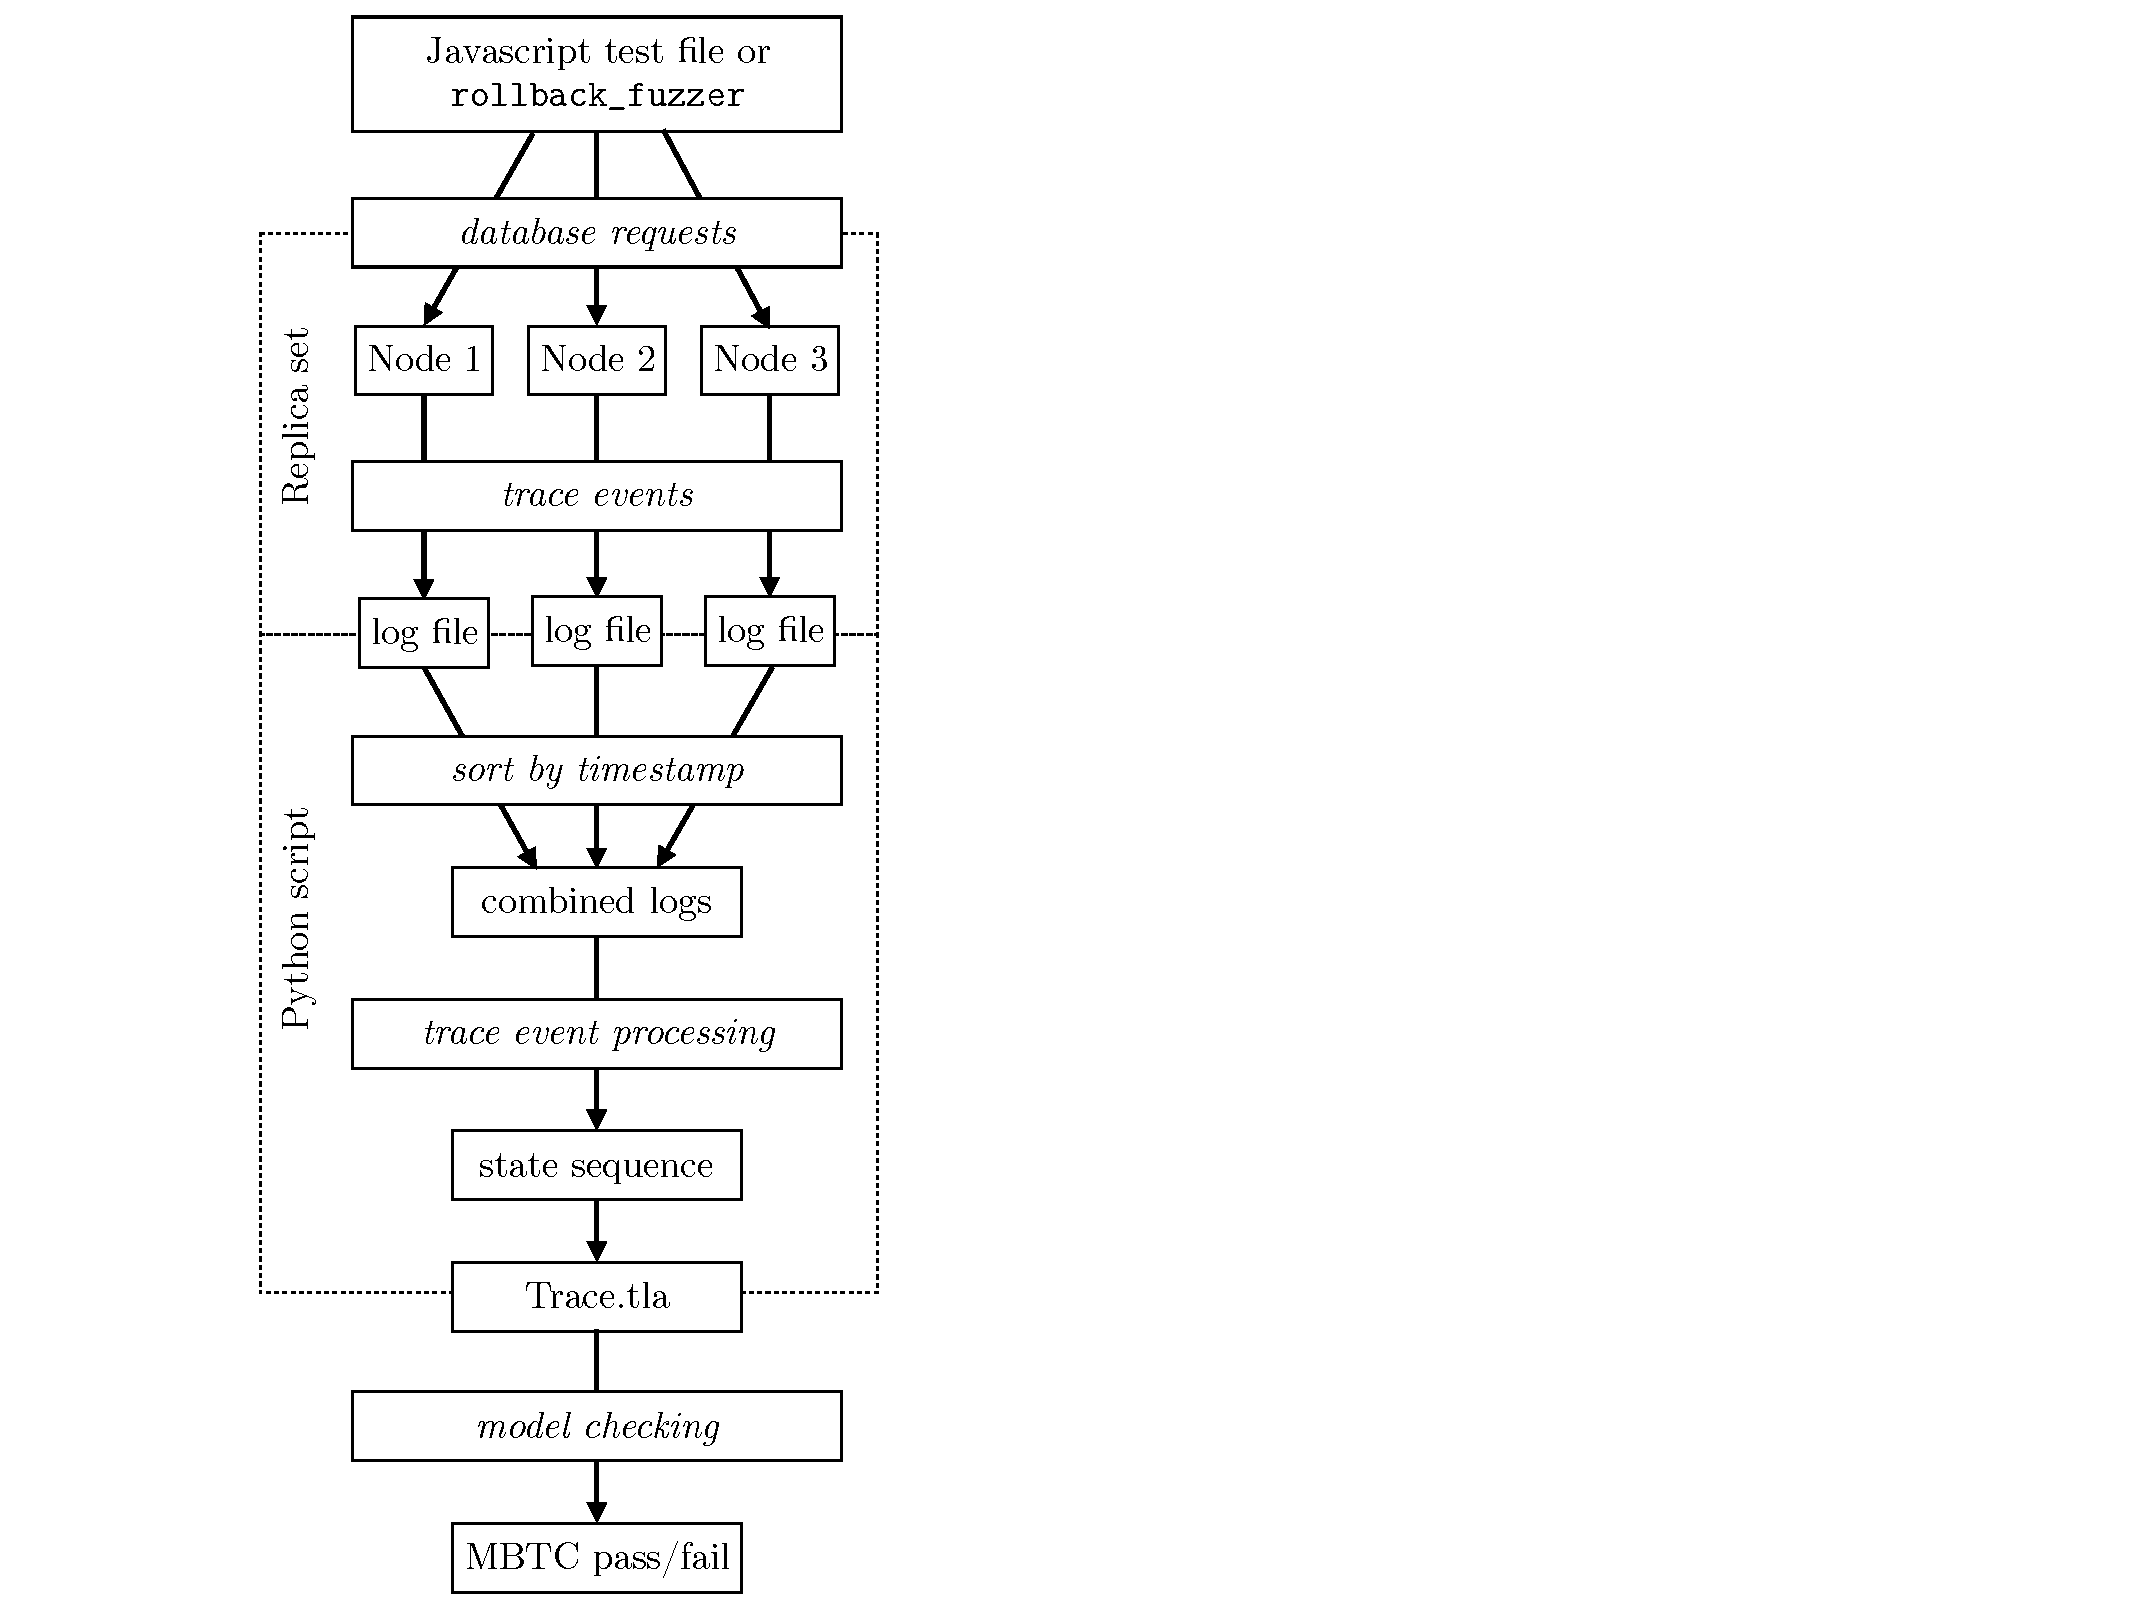
\includegraphics[width=\textwidth]{MBTC-pipeline.pdf}
\caption{MBTC data pipeline}
\label{figure:MBTC-pipline}
\end{figure}

Prior to our research, there were 423 integration tests handwritten in JavaScript that target our replication protocol, and 23 randomized test suites that pause, disconnect, and terminate servers while the replica set is performing regular operations. 
Our goal was to capture traces from all our tests and check them against all our specifications.

For our prototype we chose one specification, a 345-line TLA+ file called \texttt{RaftMongo.tla} in the MongoDB Server repository \cite{MongoGitHub}.
The specification's primary concern is to describe the gossip protocol by which replicas learn the \textit{commit point}: the newest oplog entry that has been replicated by a majority.
This specification is based on Diego Ongaro's TLA+ specification for Raft \cite{Ongaro14TLA+Raft}.
The same as in Raft, replicas in our specification can assume roles Leader or Follower. Time is divided into consecutively numbered election terms. A new term begins whenever a replica calls for an election to choose a new leader.
One difference from Raft is that the MongoDB Server's replication protocol is a pull protocol whereas Raft is a push protocol; the MongoDB Server's follower nodes request oplog entries from the leader or other nodes, rather than the leader sending entries to followers.
\texttt{RaftMongo.tla} is very high-level with few state variables and invariants in order to focus on how the commit point is gossiped. 
Unlike Ongaro's work, our specification does not explicitly model messages passed between nodes.

Each replica's state is modelled with four variables:

\begin{itemize}[itemsep=-0.5ex]
\item \texttt{role}: ``Leader'' or ``Follower''
\item \texttt{term}: Newest election term the replica knows
\item \texttt{commitPoint}: Newest majority-committed oplog entry it knows
\item \texttt{oplog}: Contents of its oplog
\end{itemize}

There are seven named state transitions in the specification:

\begin{itemize}[itemsep=-0.5ex]
\item \texttt{AppendOplog}: A node receives entries from any node
\item \texttt{RollbackOplog}: A node removes divergent entries
\item \texttt{BecomePrimaryByMagic}: A node is elected leader instantaneously---the election protocol is abstracted away
\item \texttt{Stepdown}: A leader becomes a follower
\item \texttt{ClientWrite}: A leader executes write operations
\item \texttt{AdvanceCommitPoint}: The leader advances the commit point
\item \texttt{UpdateTermThroughHeartbeat}: A node learns the election term from any node
\item \texttt{LearnCommitPointWithTermCheck}: A node learns the commit point from any node
\item \texttt{LearnCommitPointFromSyncSource\-Never\-Beyond\-Last\-Applied}: A node learns the commit point from a more up-to-date node
\end{itemize}

% on master, git hash 12782d
% 5398516 states generated, 371,368 distinct states found, 0 states left on queue.
% The depth of the complete state graph search is 21.
% The average outdegree of the complete state graph is 1 (minimum is 0, the maximum 13 and the 95th percentile is 3).
% Finished in 13min 45s at (2020-02-08 07:54:22)

% on https://github.com/ajdavis/mongo/tree/count-original-raftmongo-states with siyuan's spec from https://raw.githubusercontent.com/visualzhou/mongo-repl-tla/master/RaftMongo.tla:
% 263971 states generated, 42,034 distinct states found, 0 states left on queue.
% The depth of the complete state graph search is 21.
% The average outdegree of the complete state graph is 1 (minimum is 0, the maximum 8 and the 95th percentile is 3).
% Finished in 02s at (2020-02-08 08:37:12)

When we configure this specification with 3 replicas and constrain the model checker to at most 3 terms and oplogs up to 3 entries long, TLC successfully model-checks it and discovers 371,368 distinct states.
TLC validates an invariant that committed writes are not rolled back and a temporal property that the commit point is eventually propagated.

% Reverting logging in commit bcae9e67774088 made 617 deletions,
% minus 42 are JS, 5 are SCons, leaves 570 C++
We wrote a C++ procedure \texttt{logTlaPlusTraceEvent}, enabled only in testing, which used our logging framework to emit as JSON the values of the four state variables above.
Then we located code paths in the MongoDB Server corresponding to the seven state transitions and added calls to this procedure.

MBTC with a distributed system requires a partial order of trace events; we achieved a strict order by running all processes on one machine and sleeping before logging the trace event.
Since all log messages include the current timestamp with millisecond precision, it was sufficient to sleep until the system clock's millisecond digit changed (Figure \ref{fig:millisecond_sleep}). (Jard et. al. describe a more general solution with vector clocks \cite{Jard94GeneralApproachToTraceChecking}.)

\begin{figure}
\begin{verbatim}
PROCEDURE logTlaPlusTraceEvent(event) {
    /* Timestamp has millisecond precision */
    Timestamp beforeTime = getCurrentTimestamp()
    Timestamp afterTime = getCurrentTimestamp()
    while (afterTime == beforeTime) {
        sleep 1 millisecond
        afterTime = getCurrentTimestamp()
    }

    assert(afterTime > beforeTime,
           "Clock went backwards")

    log(event, afterTime)
}
\end{verbatim}
\caption{Pseudocode for \texttt{logTlaPlusTraceEvent}}
\label{fig:millisecond_sleep}
\end{figure}


% Run on Jesse's workstation at commit https://github.com/ajdavis/mongo/commit/95f70b
% python3 buildscripts/resmoke.py --suites=replica_sets --storageEngine=wiredTiger --continueOnFailure --storageEngineCacheSizeGB=1 --alwaysUseLogFiles --jobs=16
% [resmoke] 2020-01-28T11:28:13.268-0500 Summary of replica_sets suite: 423 test(s) ran in 54885.49 seconds (303 succeeded, 0 were skipped, 120 failed, 0 errored)

We enabled tracing for our 423 handwritten JavaScript tests. 
Of these, 120 failed due to incompatibilities with tracing. 
(Section \ref{subsubsec:mbtc_impl_discrepencies} describes these incompatibilities.)
In total, these tests produced 42,262 trace events. 
We also selected one of our randomized tests, called \texttt{rollback\_fuzzer}, for MBTC. 
This test orchestrates network partitions which cause replicas to temporarily diverge and then to roll back writes in order to re-synchronize when the partitions are healed.
Random CRUD and DDL operations are run against leader nodes in the set to test that, with high probability, all combinations of operations and their behavior on rollback work consistently.
Nodes are also randomly restarted to test that clean and unclean restarts during rollback procedures do not lead to data corruption.
A representative run of \texttt{rollback\_fuzzer} produced 2,683 trace events.

% How much TLA+ statement and space coverage did today's rollback_fuzzer suite hit?
% from a given run of the suite, 1 JS file, 3 nodes, 2683 trace events
% Follow instructions on https://github.com/tlaplus/tlaplus/issues/413
We wrote a Python script \cite{ReplTraceChecker} to post-process trace logs. 
The script merges the replicas' logs and sorts them by timestamp to obtain a sequence of trace events. 
Each event describes the state of only \textit{one} replica at the moment after it executes a state transition.
In order to construct a sequence of states describing the \textit{entire} replica set, the script begins with a known initial state, combines it with the first trace event to determine the next state, and so on. 
The logic to combine a current state $S$ with a trace event $E$ from replica node $N$ to produce next state $S'$ is as follows:

\begin{itemize}[itemsep=-0.5ex]
\item \texttt{role}: The script assumes there are never two leaders at once (although this is unrealistic, see Section \ref{subsubsec:mbtc_impl_discrepencies}). Thus if the role of $N$ in $E$ is ``Leader'' then its role in $S'$ is ``Leader'' and all others' roles in $S'$ are set to ``Follower''. If $N$ had role ``Leader'' in $S$ and now has role ``Follower'' in $E$, its role in $S'$ is ``Follower'' and the other nodes' role values are unchanged. 
\item \texttt{term}: The term of $N$ in $S'$ is replaced with its term in $E$. The other nodes' terms are unchanged.
\item \texttt{commitPoint} and \texttt{oplog}: Similar to term.
\end{itemize}

For example, in Figure \ref{figure:event-processing}, the replica set's current state has Node 1 as the leader in term 1. 
The script processes a trace event from Node 2 announcing it has become leader in term 2, arriving at the next state.

\begin{figure}
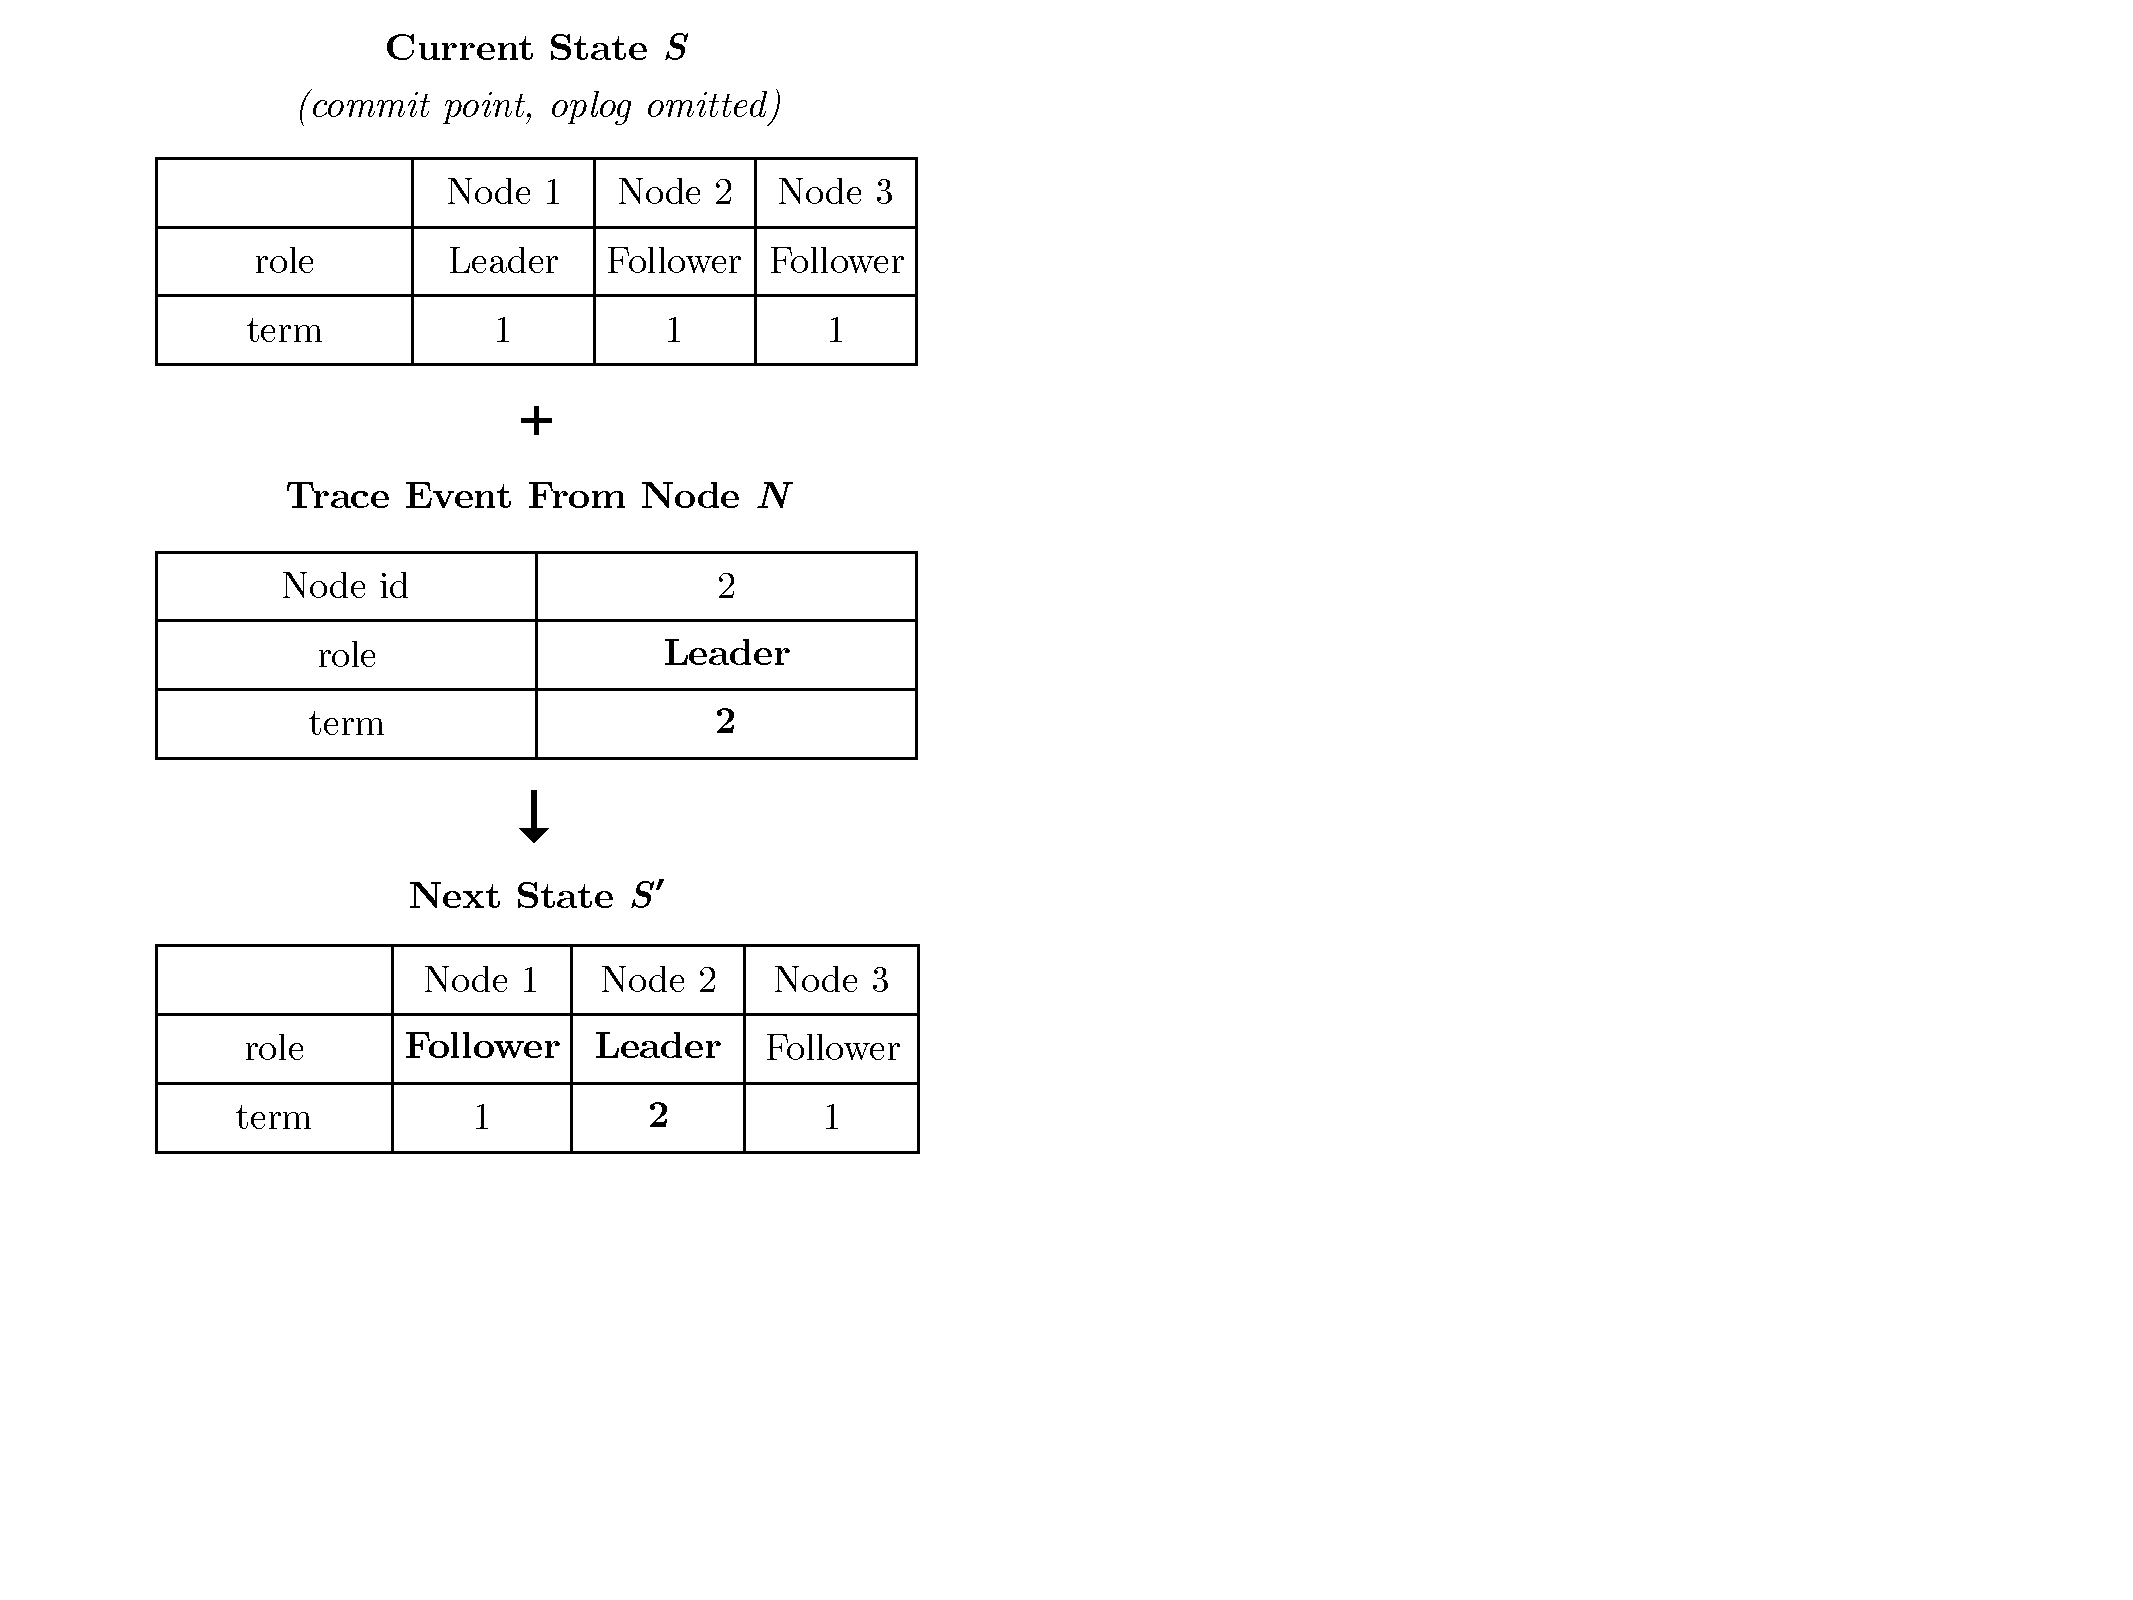
\includegraphics[height=32em]{event-processing.pdf}
\caption{Trace Event Processing}
\label{figure:event-processing}
\end{figure}

\begin{figure}
% java -cp '/Applications/TLA+ Toolbox.app/Contents/Eclipse/tla2tools.jar' tla2tex.TLA -style tlatex -shade -nops Trace.tla
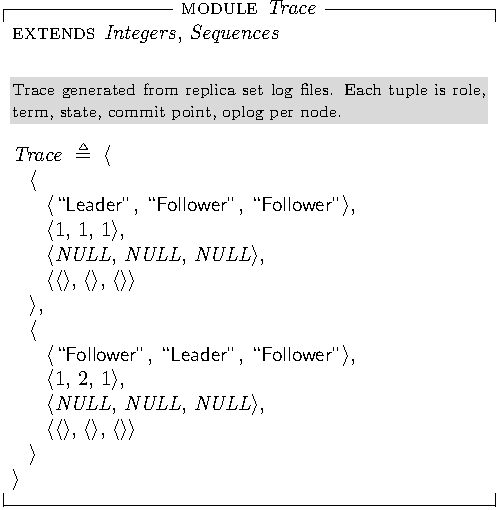
\includegraphics{Trace.pdf}
\caption{State sequence as TLA+ tuple (simplified)}
\label{fig:state-sequence}
\end{figure}

Once the script constructs this sequence of states, it implements MBTC following a method proposed by Pressler \cite{Pressler18VerifyingSoftwareTracesTLAPlus}: it generates a TLA+ module called \texttt{Trace.tla} which includes the sequence of states (Figure \ref{fig:state-sequence}), and uses TLC to check that the sequence is permitted by the \texttt{RaftMongo.tla} specification.
The entire data pipeline can be seen in Figure \ref{figure:MBTC-pipline}. 
It was implemented by two engineers in two and a half months.

\begin{center}
\begin{tabular}{ | m{11em} | m{5em}| m{6em} | } 
\hline
Task & Effort & Lines of Code \\  
\hline
Event tracing & 4 weeks & 570 C++ \\ 
Update RaftMongo.tla & 3 weeks & 252 TLA+\\ 
Python post-processor & 3 weeks & 484 Python \\ 
\textbf{Total} & \textbf{10 weeks} & \\
\hline
\end{tabular}
\end{center}

\subsection{Analysis}
\label{subsec:mbtc_analysis}

% Probably irrelevant: We considered either a Java harness that fed trace inputs to the TLC internal API, and we tried Pressler's method. Since the former was not fully implemented in Java for us, and the latter already works and includes nice Toolbox diagnostics, we stuck w/ the latter. We also considered Pressler's suggestion of using his method w/ a custom operator that avoids passing through TLA+ tuples as the repr of the trace, we didn't need to do that either.

% Counting from Oct 10, 2019 https://github.com/mongodb-labs/repl-trace-checker/commit/5c96b44d to 
% Jan 10+.
We had intended to trace-check some or all our specifications against traces from our 423 handwritten tests and 23 randomized tests, deploy the trace-checker to our continuous integration system, and measure accumulated state space coverage over all tests. 
We had hoped that the marginal cost of checking each specification after the first would decrease.
Had we achieved this, we would have built much of the test infrastructure required for eXtreme Modelling.
However, we applied trace-checking to only 5 handwritten tests and one randomized test. 
Only one handwritten test generated traces that passed the trace-checker; the other 4 produced traces that violated the specification due to two implementation discrepancies (see the discussion of initial sync and term in Section \ref{subsubsec:mbtc_impl_discrepencies}). 
We did not deploy to continuous integration nor measure coverage. 
The effort to implement MBTC proved so costly for us that we abandoned the project after two and a half months of engineering effort. 
We faced complexities with concurrency and locking, discrepancies between our models and implementation, and incomplete support in TLC. 
With further effort we might have achieved MBTC for one specification, but we estimated that the marginal cost of checking each additional specification would approach the cost of the first.

In the following sections we describe our issues trace-checking \texttt{RaftMongo.tla}, argue that additional specifications would be just as costly, and offer advice for future implementers of MBTC.

\subsubsection{Visibility, hierarchical locking}
\label{subsubsec:mbtc_locking}

\textbf{Visibility}: When we began to add tracing to the MongoDB Server, we realized each trace event must be logged after it has occurred, but \textit{before} the change is visible to other replicas. 
For example, when a leader receives a write from a client application and creates an oplog entry, it must log the \texttt{ClientWrite} event after the entry has appeared in its own oplog, but before any followers can replicate the entry and log an \texttt{AppendOplog} event for it. 
If a follower logged an \texttt{AppendOplog} event with an earlier timestamp than the leader's \texttt{ClientWrite} event, the trace would violate the causal relationship described in the specification. 
To ensure each state change was logged before it became visible to other processes, our logging code had to hold one or more locks.

\textbf{Hierarchical locking}: Formal specifications of distributed systems algorithms, such as Raft, model a concurrent system of interacting processes, but they typically model each process as single-threaded. 
Production database systems such as the MongoDB Server, however, almost always have high intra-process concurrency and employ some degree of hierarchical locking \cite{Gray76SharedLocks}. 
The MongoDB Server specifically combines hierarchical locking with storage-engine Multi-Version Concurrency Control (MVCC), C++ latches, and higher level concurrency control primitives like futures.
It may not be feasible to log a consistent snapshot of such a process's state at the moment of a trace event.

% _tlaPlusRaftMongoEvent_inlock's caller has replcoord mutex, the fn gets Global IS,
% DB IS, and Collection IS locks for local.oplog.rs.
% more details in https://mongodbcr.appspot.com/536420002/, particularly patch set 9
% map locks A, B, C to RSTL, Global, replcoord mutex.

To implement MBTC for \texttt{RaftMongo.tla}, a replica must include the contents of its oplog with each trace event, but acquiring the locks to obtain a snapshot of the oplog proved difficult. 
Suppose our \texttt{logTlaPlusTraceEvent} procedure (Figure \ref{fig:logTlaPlusTraceEvent}) must acquire locks A, B, and C, in that order, to read the oplog.
Consider a procedure \texttt{becomeLeader} that acquires locks A and C, then changes the replica's role to Leader. 
If we add a call from \texttt{becomeLeader} to \texttt{logTlaPlusTraceEvent}, the latter must acquire lock B, but this is the wrong order and risks deadlocking with other threads.
If \texttt{becomeLeader} first \textit{dropped} lock C, then acquired locks B and C, that would be the correct order.
But dropping lock C could allow a thread servicing an external request to communicate the node's new role to another process, thus making the role change \textit{visible} and violating the visibility rule described above.
General solutions are unpalatable: callers of \texttt{logTlaPlusTraceEvent} could be responsible for acquiring all the locks it will need, but this encodes intimate knowledge about \texttt{logTlaPlusTraceEvent} into its callers, and it significantly alters the system's behavior under test.

\begin{figure}
\begin{verbatim}
PROCEDURE becomeLeader() {
    acquire Lock A
    acquire Lock C
    role := Leader
    logTraceEvent()
}

PROCEDURE logTlaPlusTraceEvent() {
    /* Wrong acquisition order if called by
       becomeLeader, risks deadlock */
    acquire Lock A if not yet acquired
    acquire Lock B if not yet acquired
    acquire Lock C if not yet acquired
    read oplog
    /* Remainder of procedure as in Fig. 4 */
}
\end{verbatim}
\caption{Pseudocode for a replica becoming a Leader}
\label{fig:logTlaPlusTraceEvent}
\end{figure}

Solving both the visibility and the locking challenges, for each of the seven named state transitions in \texttt{RaftMongo.tla}, was the single most difficult aspect of our MBTC implementation, costing roughly a month of engineering effort. 
Eventually we discovered code locations that obeyed each transition's visibility requirements.
We managed to avoid the need for acquiring locks out of order by exploiting the MongoDB Server's MVCC features: our storage engine can serve reads from an stale snapshot of the oplog, instead of locking the oplog to read its current contents.
Fortunately, in each location where \texttt{logTlaPlusTraceEvent} could not acquire the locks needed to read the current oplog, an stale snapshot was permitted by the specification.
In each code location where the specification required the most recent oplog, on the other hand, it was possible to lock it.

% Gravell: "3.3 Model-Based Trace-Checking
% To provide us with traces, we wrote a generic “trace bean” for capturing key transitions in a common database.
% Trace points were easily identified as a result of the close correspondence between top-level model and
% implementation. By hand we added trace beans and tracing code at each such point. Thereafter, each execution
% of the system automatically added to our tracing database. It was now easy to extract traces using SQL queries,
% and a small amount of scripting code, to extract and transform traces into forms that can be model-checked by
% Spin or ProB [14]."

In contrast to our difficulties adding tracing to the MongoDB Server, Gravell et. al. \cite{Gravell11ConcurrentDevelopmentOfModelAndImplementation} emphasize how easily they added tracing.
We believe their task was easier because 1) their application was a small prototype, 2) they had deliberately written their specification and implementation to closely correspond (see Section \ref{subsubsec:modelling_for_trace_checking}), and 3) their application did not support the complex intra-process concurrency of a typical database.
We were surprised at the difficulty of adding tracing to the MongoDB Server, both because it had been easy for Gravell et. al. and because we had not anticipated how visibility and locking would complicate our code.
We expect any MBTC implementation for a concurrent database would encounter similar complexities with hierarchical locking and visibility of state changes.

\subsubsection{Implementation discrepancies}
\label{subsubsec:mbtc_impl_discrepencies}

\textbf{Arbiters}: MongoDB Server replicas can be configured as \textit{arbiters} which vote in elections but have no data. 
\texttt{RaftMongo.tla} does not model arbiters and we did not implement tracing for them; arbiters crash when tracing is enabled.
This was trivial to understand and to ignore, but gave us a hint that our specs did not describe our implementation in as many cases as we wanted.

\textbf{Initial sync}: The second discrepancy was in the behavior of \textit{initial sync}, the process a follower uses to obtain a copy of the data and oplog when added to the replica set.
Trace-checking the output of \texttt{rollback\_fuzzer} immediately reproduced a known violation of the specification: our implementation considers an oplog entry to be majority-committed once a quorum of nodes, including initial-syncing nodes, has replicated it.
However, initial-syncing nodes should not be considered quorum members because their oplog entries are not durable until their initial sync completes.
We excluded this behavior from \texttt{RaftMongo.tla} when we first wrote it.
We did not have MBTC in mind, so we deliberately wrote an idealized specification with the intention to eventually bring our implementation into conformance.
When MBTC caught this violation, it increased our confidence in trace-checking; however, it was not an acceptable outcome.
The violation came only 4 steps from the trace's start and left the remaining 2,683 steps unchecked.

To permit \texttt{rollback\_fuzzer} to pass trace-checking, we could 1) fix the implementation of initial sync sooner than planned, 2) avoid triggering the non-conforming behavior in testing, 3) update the specification to match today's implementation, or 4) post-process the traces to simulate a conformant implementation.
Fixing this particular violation would require more substantial work and is already scheduled for a future release.
Instead, we chose solution 2 and modified \texttt{rollback\_fuzzer} to ensure all followers were fully synced before the test began any writes.

\textbf{Two leaders}: Similarly, although \texttt{RaftMongo.tla} assumes there is only one leader at a time, two leaders can in fact co-exist briefly. This is an unavoidable consequence of our protocol and Raft-like protocols in general.
Again we chose solution 2, and avoided tests exhibiting this behavior.

\textbf{Term}: Other discrepancies required solution 3, updating the specification. 
For example, \texttt{RaftMongo.tla} originally modelled the election term as a single global number known by all replicas.
This simplification was reasonable at the time because the election term was not the specification's original focus. 
However, in actuality, new election terms are gossiped among replicas and each may learn of the new term at a different time.
MBTC required us to make the specification more complex to match reality. 
We chose to update the specification to resolve this and many other discrepancies: over the course of our research we added or changed 252 of the 345 lines of TLA+ in \texttt{RaftMongo.tla}, costing 3 weeks of effort.

\textbf{Copying the oplog}: In several cases we chose solution 4, post-processing the logs to simulate conformance. For example, in \texttt{RaftMongo.tla}, when a node performs an initial sync, it copies the leader's entire oplog.
In the implementation, a new node copies only recent entries.
The \texttt{RaftMongo.tla} behavior more closely matches the Raft protocol that inspired it, and makes it simpler to express invariants such as ``an entry is committed after it is replicated to a majority of nodes' oplogs.''
Making the implementation conform would discard a useful optimization, and updating the specification would have required substantial effort.
Instead we resolved the discrepancy by adding logic to our Python script that filled in the missing entries while it generated the state sequence.
Such an intrusive modification made us concerned that a mistake in the Python script might mask a harmful transcription bug in the MongoDB Server code.
On the other hand, choosing solution 3 and adding detail to the specification might explode the state space and make model-checking intractable.

Each discrepancy we discovered through MBTC required us to judge which of the four solutions to employ. 
Ideally, when an organization practices eXtreme Modelling, they resolve each MBTC failure either by fixing the implementation or, if the failure is not a bug, by updating the specification.
In practice, we often concluded it was expedient to work around violations.
We chose to avoid the non-conforming behavior (solution 2) or to simulate a conformant behavior (solution 4) depending on which took less effort and least undermined our confidence in the test.
Unfortunately, our choices were based on estimates and speculation.

\subsubsection{Modelling for trace-checking}
\label{subsubsec:modelling_for_trace_checking}

There appears to be a conflict between writing a specification for documenting and model-checking a design and writing one that can be trace-checked.

We tried to implement MBTC with models that had been written for documentation and model-checking, but we found that MBTC is only practical if the specification is written with MBTC in mind.
If we began again, we would rewrite our specifications to closely correspond to the implementation.
The specification's major components would be structured similarly to the implementation's, and critical sections of the implementation would correspond with single actions in the specification.
In the case of multi-step events such as elections, we would model them with multiple actions, instead of expressing them as instantaneous single actions as we did with \texttt{BecomePrimaryByMagic} in \texttt{RaftMongo.tla}.
We would faithfully model the flaws in the implementation if we did not plan to fix them immediately.

We would rewrite our specification to model events that are easily observed in the implementation: for example, we might model protocol messages, akin to the original Raft specification.
We would try to avoid modelling state that is difficult to snapshot, especially if it is protected with complex locking.
If some state in the specification cannot be logged by the implementation, Pressler proposes a \textit{refinement mapping} technique \cite{Pressler18VerifyingSoftwareTracesTLAPlus}, in which TLC checks whether there is any sequence of the values that are missing from the trace that would permit the trace to match a behavior of the specification.

Most of these changes in our modelling style would be unobjectionable.
However, there is the danger that a less abstract specification has a state space too large to model-check in reasonable time.
The limited changes we made to \texttt{RaftMongo.tla} increased the state space from 42,034 states to 371,368, and model-checking time from 2 seconds to 14 minutes.
To complete our MBTC project would have required a more detailed specification, or applying Pressler's refinement mapping technique, both of which would threaten to explode the state space even more.

\subsubsection{Tooling and TLC}
\label{subsubsec:mbtc_tla_tlc}

Tool support for MBTC with TLA+ and TLC is a work in progress. 
Pressler's method worked well to check traces of hundreds of events, but for thousands of events it was impractically slow. 
Pressler proposed, and Markus Alexander Kuppe has begun to implement, features to check long traces by bypassing the TLA+ parser in favor of a special-purpose Java extension to TLC \cite{TLAPlusIssue413}. 
MBTC with TLA+ will be more convenient once these features are finalized and released, with publicly available examples. 
Another missing feature is the ability to combine state-space coverage reports over multiple TLC executions on different traces, which would permit engineers to calculate the total coverage achieved by deploying MBTC to continuous integration.

\subsubsection{Marginal cost of trace-checking a specification}
\label{subsubsec:marginal_cost}

Our experience with \texttt{RaftMongo.tla} convinced us that trace-checking additional models would be nearly as costly as the first.
For example, we imagined a scenario in which we had succeeded at trace-checking \texttt{RaftMongo.tla} and we moved on to \texttt{Locking.tla} \cite{LockingTLA}, which models aspects of the MongoDB Server's lock hierarchy.
Once again we would begin with highly abstract specification written for documentation and model-checking, and we would repeat the effort of adding detail and resolving discrepancies to make the specification suitable for MBTC.
The state variables of \texttt{Locking.tla} are disjoint from those modelled by \texttt{RaftMongo.tla}, so there would be little code reuse in the tracing implementation or the post-processing script.
The locking specification applies only to one process, not to an entire replica set, so the log post-processing script would be simpler for \texttt{Locking.tla} than for \texttt{RaftMongo.tla}; however, this difference would further preclude code reuse.

We canceled the MBTC project because we had achieved disappointingly little utility from our efforts, and our revised estimate of the marginal cost made it clear that the project was not worthwhile.

% -------- scrapbook ------------
% what does MBTC prove?
% Advantage of MBTC over other tests is that implementation tests can't prove liveness, unless you run them forever. TLA+ specs can be checked for liveness, and if the impl matches the spec, the impl might also not have liveness bugs.

% impl is a subset of the spec => if the spec is safe, the impl is safe
% but we can't test to the point where we know that impl is a subset of the spec
% we only know that tested behavior is a subset of the spec

% FALSE: impl is a subset of the spec => if the spec has no liveness bugs, the impl has no liveness bugs
% the impl might lack spec behaviors that are required for liveness

% ********************************************************************
% ****************** MBTCG *******************************************
% ********************************************************************
\section{Model-Based Test-Case Generation}
\label{sec:model_based_test_case_generation}

Architectural decisions for MongoDB Realm Sync have led us to re-implement the server in Golang while keeping the clients in C++. The MongoDB Realm Sync code base originally ensured the client's and server's behavior were identical by sharing the same C++ code. Now that there are two implementations, it is paramount they resolve conflicts identically. Designing OT functions that ensure peers converge to the same data is already challenging and error-prone \cite{Imine03ProvingCorrectnessOfTransformationFunctions, Imine06FormalDesignAndVerificationOfOT, Randolph13OnConsistencyofOTApproach}; implementing it the same way twice is even more difficult.

Model-based test-case generation (MBTCG) \cite{Gravell11ConcurrentDevelopmentOfModelAndImplementation} provided means to confidently assess whether parity had been achieved while both the C++ and Golang code bases were under active development. We wrote a new TLA+ specification for this purpose and used the state space explored by the TLC model checker to generate C++ and Golang test cases for aspects of the OT algorithm. These test cases can be automatically generated and run after any change to the model, and ensure that both the C++ and Golang implementations make appropriate changes to maintain equivalence with each other.

% Outline of sections to follow: (doing them in this order tells the story of how the model-based testing happened chronologically and feels like the most natural way to split up the story)
% 1. Transcribed from C++ to TLA+. Ran the model checker, found issues.
% 2. C++ code generation, fine to mention stats of # test cases and lines of C++ code rather than in separate "Analysis" subsection.
% 3. Golang code generation. (this hasn't been implemented yet)

% TODO: We should double check with Drew D. what the name of the product and what the name of the team are (or at least what we're calling them externally).
MongoDB Realm Sync has 19 distinct operations which can be performed on a group of tables, an individual table, an object, or a list of values. These include operations such as deleting a table, creating a new object in a table, setting the property of an object, and inserting a new element into a list. Each type of operation must define how it merges with all other types of operations. This yields $19 (19 + 1) / 2 = 190$ merge rules needing to be defined with the remaining $19^2 - 190 = 171$ merge rules able to be inferred by symmetry. Approximately three-quarters of the merge rules have trivial implementations where the incoming operation is applied unchanged by both peers.

The most complex merge rules are for the six array-based operations:

\begin{itemize}[itemsep=-0.5ex]
  \item \texttt{ArraySet}: replacing the value of an existing element
  \item \texttt{ArrayInsert}: inserting a new element at a position within the list, or growing the size of the list by one
  \item \texttt{ArrayMove}: moving an element from one position to another
  \item \texttt{ArraySwap}: swapping the position of two elements
  \item \texttt{ArrayErase}: removing an element from the list
  \item \texttt{ArrayClear}: removing all of the elements from the list
\end{itemize}

The $6 (6 + 1) / 2 = 21$ merge rules for these six operations are implemented in approximately 1,000 lines of C++ code.

% TODO: Do some LaTeX thing to make figure placement sane.
\begin{figure}
\begin{verbatim}
DEFINE_MERGE(ArrayErase, ArraySet)
{
  if (same_array(erase_op, set_op)) {
    // LCOV_EXCL_STOP
    if (set_op.ndx == erase_op.ndx) {
      // CONFLICT: Update of a removed element.
      // RESOLUTION: Discard the ArraySet
      // operation.
      set_op.discard();
    }
    else if (set_op.ndx > erase_op.ndx) {
      set_op.ndx -= 1;
    }
    // LCOV_EXCL_START
  }
}
\end{verbatim}
\caption{C++ code for merging \texttt{ArrayErase} and \texttt{ArraySet} operations}
\label{fig:cpp_erase_set_merge}
\end{figure}

\subsection{Writing the TLA+ specification}
\label{subsec:mbtcg_tlaplus}

MongoDB's Realm Sync Team wrote a TLA+ specification for these array-based operations to assess the soundness of the existing C++ implementation and to provide a means for exhaustively generating test cases for a new Golang implementation.

% TODO: Should we add a description of the variables in the TLA+ specification?

% Max likes the following phrase but it no longer has a sensible place to go.
% for conditionally adjusting the index numbers

% TODO: Do some LaTeX thing to make figure placement sane.
\begin{figure}
% java -cp '/Applications/TLA+ Toolbox.app/Contents/Eclipse/tla2tools.jar' tla2tex.TLA -style tlatex -shade -nops array_ot_invariant.tla
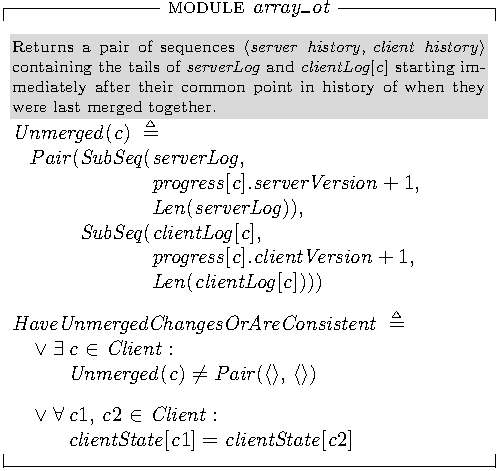
\includegraphics{array_ot_invariant.pdf}
\caption{TLA+ invariant for MongoDB Realm Sync}
\label{fig:tlaplus_realm_sync_invariant}
\end{figure}

Writing the TLA+ specification took approximately 40 hours over the course of two weeks. The TLA+ specification was written by copy-pasting the C++ code and manually updating the syntax to be valid TLA+. The merge rule for two \texttt{ArrayInsert} operations was written first along with the \texttt{HaveUnmergedChangesOrAreConsistent} invariant (see Figure \ref{fig:tlaplus_realm_sync_invariant}).
The merge rules for each subsequent operation type were then added with runs of the TLC model checker occurring in between each group of merge rules being added.
The TLC model checker found transcription errors multiple times during this process. The counterexample produced was then manually analyzed by associating the branches taken in the series of if-statements in the C++ code with the nested \texttt{IF} and \texttt{CASE} expressions taken in the TLA+ specification.

This transcription process was challenging in two ways. First, the C++ code relies on mutable variables for expressing how the incoming operations must be modified to be correctly applied by the non-originating peer, whereas TLA+ variables cannot be mutated in the same way. Second, the order in which clients perform operations locally and then later merge with the server doesn't impact their final state, and, if left unconstrained, would quickly lead to a state space explosion.

% TODO: Do some LaTeX thing to make figure placement sane.
\begin{figure}
% java -cp '/Applications/TLA+ Toolbox.app/Contents/Eclipse/tla2tools.jar' tla2tex.TLA -style tlatex -shade -nops array_ot_merge_example.tla
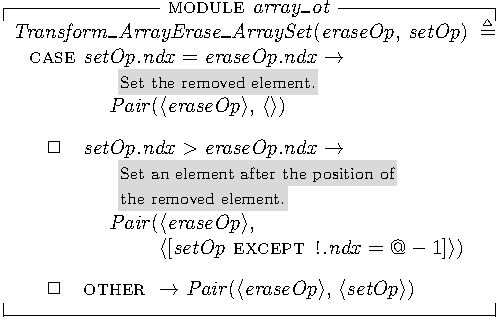
\includegraphics{array_ot_merge_example.pdf}
\caption{TLA+ code for merging \texttt{ArrayErase} and \texttt{ArraySet} operations}
\label{fig:tlaplus_erase_set_merge}
\end{figure}

\subsubsection{Handling C++ mutability and flow control}

% TODO: Are there papers we could cite for these sort of challenges with TLA+?
TLA+ isn't a general-purpose programming language. \emph{Operators} in TLA+ (which behave most closely to a function in a general-purpose programming language) lack the concept of reassigning an argument or having multiple statements as in C++.
While PlusCal offers an imperative syntax, it only supports reassigning state variables---and not arguments within an operator---because it still transpiles to TLA+.
As shown in Figure \ref{fig:cpp_erase_set_merge}, the C++ variable \texttt{set\_op} is mutated to produce the version of these operations to be applied on the non-originating peer. This mismatch between the two languages makes it more difficult to formalize a C++ source of truth into a TLA+ specification, especially in the presence of nested if-statements. Additionally, a series of multiple if-statements must be transcribed to explicitly define all branch combinations that may or may not be taken consecutively. Fortunately, the TLC model checker was readily able to catch human transcription errors as safety violations. Some examples of transcription errors were forgetting to substitute the updated index number in later comparisons, or entirely forgetting to embed a deeply-nested or later occurring if-statement as another nested \texttt{IF} or \texttt{CASE} expression in TLA+.

\subsubsection{Constraining the state space}

The state constraint was progressively refined as the TLA+ specification was being implemented in order to reduce the run-time required by the TLC model checker. One simplification was a \texttt{MergeAction} operator which simultaneously uploads any changes from the client and downloads any changes from the server. Modelling these as distinct actions would only have been beneficial when explicitly modelling time. Instead, the model's purpose is to generate C++ and Golang test cases where clients perform a sequence of operations starting from the same initial array. A client performing a sequence of operations that are causally dependent on another client's sequence of operations is equivalent (in terms of both its state and history) to the former client performing the concatenation of the two sequences on the same initial array. However, a longer sequence of operations necessarily has more combinations and would lead to a state space explosion. We therefore shifted to focus on varying the initial array and restricted all clients to performing a single operation. Since the TLC model checker would explore all combinations of the clients performing a single operation, starting with a sufficiently large initial array would still enable the TLC model checker to exercise every case in the merge rules.

We artificially constrained the state space to have clients perform and merge operations in ascending order of their ID to avoid exploring redundant states. In particular, it doesn't matter which order clients 1 and 2 perform operations locally until they communicate with the server. We aren't able to define the clients as a symmetry set because the ID is used to order operations when their timestamps are equal. As mentioned previously, the specification doesn't model time, so we need at least 3 clients to capture a client merging both with an earlier operation and with a later operation.
Using the minimum of 3 clients ensures we don't increase the state space unnecessarily.
The TLC model checker was run with constraints of 3 clients each performing a single operation on an array already containing 3 elements.

\subsubsection{Results from the TLC model checker}

In addition to detecting safety violations caused by transcription errors, the TLC model checker also encountered a \texttt{StackOverflowError} due to a case in the merge rule for the \texttt{ArraySwap} and \texttt{ArrayMove} operations leading the merge function to never terminate. This issue was found to also exist in the C++ code; the bug had faithfully been transcribed from C++ to TLA+. It was surprising to discover a bug in the C++ implementation due to the maturity of the product and the amount of randomized testing it had undergone.
The discovery of this issue became the deciding factor to not support a dedicated \texttt{ArraySwap} operation in the new Golang server implementation. The \texttt{ArraySwap} operation was therefore excluded from testing for the remainder of this experiment.

Even if the model checker does not find a violation of the \texttt{HaveUnmergedChangesOrAreConsistent} invariant, this does not imply that the specification accurately describes the C++ implementation.
For example, a trivial way to achieve convergence (at the cost of user-intent preservation) would be to have every merge rule clear the contents of the array. We must test that the behavior of the specification conforms to the C++ code.

\subsection{Generating C++ test cases}
\label{subsec:mbtcg_cpp}

The state space explored by the TLC model checker provides an exhaustive set of test cases for how a given pair of operations should be transformed when applied by the non-originating peer. The TLC model checker supports writing the graph of all reachable states as a DOT file. The \texttt{-dump dot,actionlabels graph} option causes the TLC model checker to generate a graph.dot file where nodes in the graph are labeled with the state (a conjunction of assignments to all \texttt{VARIABLE}s declared in the TLA+ specification) and edges are labeled with the action taken to progress from one state to the next.

A BNF grammar for the TLC model checker's state representation was written and a parser generator for Golang was used \cite{GoccGitHub} to generate a parser for it. The state graph for a run with 3 clients each performing a single operation was then analyzed in a Golang program to generate C++ test cases composed of (1) the initial array, (2) the operations each client performed, (3) the transformed version of the operations each client applied after merging the original operations from the other clients, and (4) the final state of the array. The Golang program then produces a C++ program which uses MongoDB Realm Sync's unit test framework. The \texttt{fixture.sync\_all\_clients()} call takes the place of performing the merge action for all the clients (in the same order the TLA+ specification performs the merge).

\begin{figure}
\begin{verbatim}
TEST(Transform_Node__6971023528664242108)
{
  size_t num_clients = 2;
  TransformArrayFixture fixture{
    test_context, num_clients, {1, 2, 3}};

  fixture.transaction(0, [](TableRef array) {
    array->set_int(0, 2, 4);
  });
  fixture.transaction(1, [](TableRef array) {
    array->remove(1);
  });

  fixture.sync_all_clients();
  fixture.check_array({1, 4});

  fixture.check_ops(0, {ArrayErase{1}});
  fixture.check_ops(1, {ArraySet{1, 4}});
}
\end{verbatim}
\caption{C++ test case for merging \texttt{ArrayErase} and \texttt{ArraySet} operations}
\label{fig:cpp_test_erase_set_merge}
\end{figure}

% 4913 test cases with 3 element array, 3 clients performing 1 operation each
% 50653 test cases with 5 element array, 3 clients performing 1 operation each
For an initial array containing 3 elements and with 3 clients each performing a single operation, the Golang program generated 4,913 C++ test cases.
The coverage of the specific sections of the C++ code was measured by adding in \texttt{LCOV\_EXCL\_STOP} and \texttt{LCOV\_EXCL\_START} comments within the block of the \texttt{same\_array()} condition. This was done because the TLA+ specification was designed to only exercise cases where the clients act on the same array.
The 36 handwritten C++ test cases covered 18 of the 86 branches (21\%) within the merge rules for the array-based operations.
This low percentage is excused by how MongoDB Realm Sync has relied on randomized testing to harden its implementation of the OT algorithm.
The \texttt{fuzz-transform} test executable, which uses the AFL fuzzer \cite{AFLHomepage} to produce randomized inputs that are then mapped to randomized operations, covered 79 of 86 branches (92\%) after approximately 8 million total executions.
The generated C++ test cases covered all 86 branches (100\%).


% TODO (Max): We could potentially describe a change made in the TLA+ specification to make it more useful at the expense of not exactly representing what the C++ code does.
% Elements within a list are referred to by their index number. The array-based operations make up ~1,000 lines of C++ code of conditionally adjusting index numbers to define 6 * (6 + 1) / 2 = 21 merge rules.

Achieving 100\% branch coverage and all the generated C++ test cases passing gives us confidence in the TLA+ specification conforming to the C++ code.
There may still be programming bugs in the C++ implementation stemming from undefined behavior.
However, for the well-formed inputs from the TLC model checker, we can be certain the OT algorithm converges and the C++ and Golang implementations of the merge rules for the array-based operations would always agree.
It was worth it for a single engineer to spend one month writing the TLA+ specification and implementing the C++ test case generator.

% TODO: We should probably say the 755 lines of Golang excludes the generated parser code. Not sure how to most neatly add that parenthetical to the table without upsetting the formatting.

\begin{center}
\begin{tabular}{ | m{11em} | m{5em}| m{6em} | } 
\hline
Task & Effort & Lines of Code \\  
\hline
array\_ot.tla & 2 weeks & 795 TLA+ \\
C++ test case generator & 2 weeks & 755 Golang \\
\textbf{Total} & \textbf{4 weeks} & \\
\hline
\end{tabular}
\end{center}

% ********************************************************************
% ****************** Conclusions *************************************
% ********************************************************************
\section{Conclusions}
\label{sec:conclusions}

MBTC failed because we lacked a close correspondence between the MongoDB Server implementation and \texttt{RaftMongo.tla}.
This was partly by necessity: the MongoDB Server is hundreds of thousands of lines of code; the replication protocol alone is tens of thousands of lines due to the machinery being intertwined with many other parts of the system.
Any close correspondence with the MongoDB Server's implementation would inevitably have made the spec overly complicated for its purpose, and likely it would have inflated the state space beyond what is feasible to model-check.
In the absence of a close correspondence, MBTC requires significant post-processing of traces. 
We learned that in a system of the MongoDB Server's size and complexity, post-processing is unavoidable, and should be used early and often.
Intra-process concurrency control was the main culprit that made trace-logging more difficult than expected.
Future engineers in our situation might avoid this by synthesizing trace events during post-processing: Each time the implementation executes a state transition, it might log only the state variables that can be accessed with the locks it is permitted to acquire.
The post-processing script can then complete the trace by filling in missing variables with their previous values, under the assumption that they have not changed since the previous trace event.
Of course, this assumption must hold in order for such a technique to be valid.
Synthesizing trace events may mask bugs, so it is critical to think about what kinds of bugs the MBTC effort aims to catch and what kinds are targeted by other tests.

% ensure same length columns on last page (might need two subsequent latex runs)
% To avoid the "You have called \balance in second column" warning, the following line should be for a paragraph in the first column on the last page.
\balance

Another approach is to generate traces from modules running in a unit test framework, rather from an integration test of the entire multi-process system, as we did.
Implementation modules are smaller, simpler, and non-determinism can be more easily eliminated, for example by simulating the system clock. 
The difficulties we experienced with visibility and hierarchical locking would likely be more manageable.
By testing modules in isolation, one could sacrifice realism in exchange for implementing MBTC cost-effectively.
Especially if there are multiple specifications modeling aspects of the system, as in our case, it would be appropriate to pair a specification with each implementation module.

Regardless, MBTC in a system of the Server's scale will likely require significant effort for every specification.
No initial infrastructure investment can make the marginal cost of trace-checking additional specifications cheap.

MBTCG succeeded because the specification was deliberately written with a close correspondence to the implementation, via direct transcription.
The implementation under test was a self-contained function with defined inputs and output, of approximately one thousand lines of code. 
By design of the OT algorithm, the order of clients exchanging operations they performed locally does not change the transformed version of these operations or the resulting array.
As a result of this symmetry, the specification's behaviors can be model-checked in a reasonable amount of time, and the implementation can be completely tested by a constrained set of tests that can be generated, compiled, and run in reasonable time.

MBTC and MBTCG are both promising approaches to ensuring conformance between a spec and an implementation.
In a small system, MBTCG was highly effective and accomplished its goal.
When MBTCG is possible, and when the state space is not too large, MBTCG is the gold standard of ensuring specification-implementation conformance.
If the state space becomes too large though, or if any individual test case would take too long to run, we must start sampling the space, and MBTC can be effective.
MBTC is also a good approach when the implementation's behavior is non-deterministic and cannot be forced to execute specific test sequences.
However, when the implementation becomes too large, neither may be possible without a large investment per-specification.

Future work should make both model-based testing approaches more practical.
TLC performance was an obstacle, and any improvements would be highly valuable.
Better research and tooling to post-process partial states and merge them together under certain assumptions could make the post-processing safer and easier.
More research should determine best practices for writing specifications intended to be used in model-based testing.
It should also determine best practices for logging trace events and generating test-cases from a model.
Developing tooling for whole-process snapshotting could have greatly simplified MBTC trace logging, since we could have used the snapshots to create trace events.
Research into record-and-replay debuggers \cite{OCallahan17RRDebugger} might be applicable to this area.
Making MBTC and MBTCG first-class features in TLC could have saved us a great deal of time.
The state space representation in TLC could be improved to be more easily parsed, which would have eased MBTCG.
Trace-checking could be built in where users only need to provide a trace and a specification and TLC efficiently checks the traces for them.

Going forward, we plan to continue using TLA+ to give us confidence and increase our own understanding in our complex protocols.
MongoDB Realm Sync is actively using and improving its use of MBTCG.
More teams and projects throughout MongoDB are starting to use TLA+ to gain similar benefits in their own development.
These projects may find interest in ensuring specification-implementation conformance, and this research and any further research will help us determine when the investment is worth it, and what model-based testing method we should use.

%\end{document}  % This is where a 'short' article might terminate

% ********************************************************************
% ****************** Acknowledgements ********************************
% ********************************************************************
%ACKNOWLEDGMENTS are optional
\section{Acknowledgments}
\label{sec:acknowledgments}
Many experts have advised us, proposed workarounds for obstacles, reviewed our code, and reviewed drafts of this paper, including 
David Bradford,
Mark Callaghan,
Mike O'Brien,
Siyuan Zhou,
Will Schultz,
Michael Cahill,
Simon Ulsnes,
Tess Avitabile,
Henrik Edin,
Andy Schwerin,
and Ron Pressler.
We are embarrassingly indebted to Markus Alexander Kuppe for answering our questions about TLC within minutes, and implementing features we requested within hours.

% The following two commands are all you need in the
% initial runs of your .tex file to
% produce the bibliography for the citations in your paper.
\bibliographystyle{abbrv-original-case}
\bibliography{main}  % use main.bib file
% You must have a proper ".bib" file
%  and remember to run:
% latex bibtex latex latex
% to resolve all references
\end{document}
